\documentclass[a4paper,12pt,openany]{article}

\usepackage[brazil]{babel}
\usepackage[T1]{fontenc} 
\usepackage{ae}
\usepackage[utf8]{inputenc}
\usepackage{graphicx}
\usepackage{indentfirst}
\usepackage{amstext}
\usepackage{amssymb}
\usepackage[a4paper,left=3cm,right=3cm,top=3cm,bottom=3cm]{geometry}
\usepackage{tipa}
\usepackage[colorlinks,breaklinks,urlcolor=blue,linkcolor=black]{hyperref}
\usepackage{setspace}
\usepackage{color}

%############ BACKGROUND ##################
\usepackage{eso-pic}
\newcommand\BackgroundPic{
\put(0,0){
\parbox[b][\paperheight]{\paperwidth}{
\vfill
\centering
%\includegraphics[width=.95\paperwidth,height=.95\paperheight,keepaspectratio]{o-grito.jpg}
%\includegraphics[width=.9\paperwidth,height=.9\paperheight,keepaspectratio]{o_grito_moderno.jpg}
\includegraphics[width=.9\paperwidth,height=.9\paperheight,keepaspectratio]{Grito_PB.jpg}
\vfill
}}}

%############### FONTE #####################
\usepackage[T1]{fontenc}
\usepackage[lf]{venturis} %% lf option gives lining figures as default; 
% remove option to get oldstyle figures as default
\renewcommand*\familydefault{\sfdefault} %% Only if the base font of the document is to be sans serif


\begin{document}

	\begin{titlepage}
	
	\AddToShipoutPicture*{\BackgroundPic}

        \begin{center}
            UNIVERSIDADE TECNOLÓGICA FEDERAL DO PARANÁ\\
            DEPARTAMENTO ACADÊMICO DE INFORMÁTICA\\
            CAMPUS CURITIBA
          
            \vspace{2cm}
            
            PET-ECO APRESENTA

            \vfill

            {\Huge \emph{\colorbox{black}{\color{red} NÃO ENTRE EM PÂNICO!}} }
            
          	%\includegraphics[width=.7\linewidth]{o_grito_moderno.jpg}

            \vspace{13cm}
            
            {\LARGE \textbf{\color{blue} MANUAL DE SOBREVIVÊNCIA} }

            \vfill
            
            2011
        \end{center}

	\end{titlepage}

% ************************* SUMÁRIO *******************************************
\thispagestyle{empty}
\tableofcontents

% *********************** INTRODUÇÃO ******************************************
\newpage
\section{Introdução}

Você acaba de entrar na faculdade e está totalmente perdido  ... não se desespere! Felizmente, você não é o primeiro a viver essa situação e nem será o último, então respire fundo, conte até dez e leia até o fim (se não dormir antes) esse manual. Assim talvez as coisas se tornem um pouco menos complicadas. 

Esse Manual, elaborado por integrantes do grupo PET de Engenharia de Computação, traz algumas dicas de como sobreviver a esse universo novo chamado Universidade Tecnológica. Ele foi feito para te ajudar com algumas dúvidas que são comuns entre os calouros; caso ainda se sinta confuso com relação a alguma coisa, sinta-se à vontade para procurar o PET-ECO (nos corredores ou \url{http://www.dainf.ct.utfpr.edu.br/peteco} ou ainda \href{mailto:petecoutfpr@gmail.com}{petecoutfpr@gmail.com}) e esclarecer suas dúvidas e, claro, sugerir modificações também.

% *********************** LOCALIZE-SE *****************************************
\newpage
\section{Localize-se!}

O Campus Centro da Unidade Curitiba da UTFPR é relativamente pequeno. Diferente de outras universidades, ocupa apenas uma quadra. Apesar disso, no começo, é comum não encontrar alguns lugares aonde se deseja ir.

	\begin{figure}[ht!]  \centering
		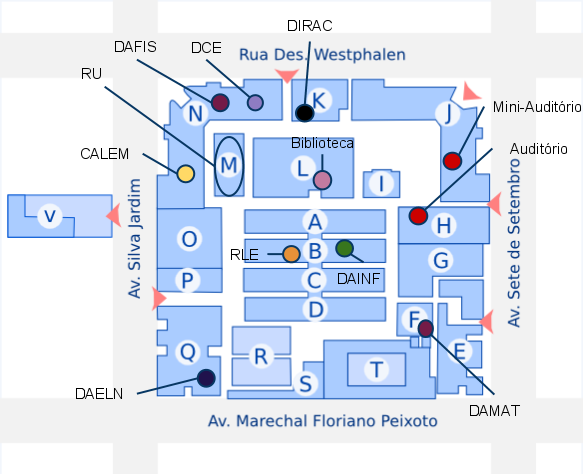
\includegraphics[scale=0.7]{mapa.png}
		\caption{Mapa do Campus Curitiba Centro}
		\label{fig01}
	\end{figure}

Neste mapa resumido, incluímos alguns lugares que consideramos importantes para os calouros do 
DAINF. São eles:

\begin{itemize}

\item \textbf{Auditório} (Bloco J)\\ aqui (e no miniauditório) acontecem diversos eventos durante o semestre.

\item \textbf{Biblioteca} (Bloco L) \\aqui você encontra além de livros didáticos e acadêmicos dissertações e teses que podem ser de grande ajuda nos estudos. Há também computadores para pesquisas pela Internet, acesso ao e-mail, site do PET, Facebook, Twitter e Orkut - entrada pelo segundo andar.

\item \textbf{CALEM} (Bloco N) (\textit{Centro Acadêmico de Línguas Estrangeiras Modernas}) \\aqui você pode obter informações sobre os vários cursos de línguas ofertados para alunos da UTFPR.

\item \textbf{DAINF} (Bloco B) (\textit{Departamento Acadêmico de Informática}) \\Aqui é, por assim dizer, o quartel-general dos alunos do departamento, você encontra os professores do DAINF e a sala de monitoria - os horários de atendimento estão disponíveis na recepção do departamento.

\item \textbf{DAELN} (Bloco Q) (\textit{Departamento Acadêmico de Eletrônica})\\ Para os alunos de Engenharia, esse é o segundo quartel-general, os laboratórios (inclusive o Laboratório Livre) e as aulas de Eletrônica acontecem nesse prédio e os professores do Departamento de Eletrônica também se encontram aqui.

\item \textbf{DCE} (Bloco N) (\textit{Diretório Central dos Estudantes} também chamado de \textbf{GECEL} devido ao \textit{Grêmio Estudantil Cesar Lattes})\\ Além de sede do DCE, aqui se encontra um serviço de fotocópias e impressões muito útil, geralmente os professores deixam materiais para cópia aqui - entre pelo térreo e desça a escada.

\item \textbf{DIRAC} (Bloco K) (\textit{Divisão de Registros Acadêmicos})\\ Secretaria geral da UTFPR. Procure para qualquer dúvida relacionado a matrícula, comprovantes e afins.

\item \textbf{Miniauditório} Ver Auditório.

\item \textbf{RLE} (Bloco B) (\textit{Rede Local de Ensino}) \\Suporte dos Laboratórios do DAINF (primeiro andar). Há também computadores no corredor, caso você queira olhar o e-mail rapidamente, verificar sua nota no Sistema Acadêmico ou elogiar aquele professor gente fina pelo Twitter.

\item \textbf{RU} (Bloco M)\\ Restaurante Universitário, aqui se come (quando dá tempo).

\item \textbf{DAMAT} (Bloco F, segundo andar) (\textit{Departamento Acadêmico de Matemática})\\ Os professores das disciplinas de Matemática (Cálculos 1, 2, 3, $10^3$, Matemáticas 1, 2, 3, $10^3$ ...) atendem aos alunos em horários pré-estabelecidos aqui.

\item \textbf{DAFIS} (Bloco N, segundo andar) (\textit{Departamento Acadêmico de Física})\\  Local de atendimento dos professores das disciplinas de Física e também laboratórios das aulas práticas de Física.

\end{itemize}

Mesmo depois dessa lista ainda não encontrou o que precisa? 

\href{http://200.134.25.110/mapa/mapa.html}{Neste link} você encontra uma relação dos departamentos/locais importantes de cada bloco!


% *********************** ACESSO À INTERNET ************************************
\newpage
\section{Acesso à Internet}

\subsection{Laboratórios}


\subsection{Wi-fi}

Sobre as senhas:
\begin{itemize}
\item Para conectar na rede wireless \textbf{WIFI-RLE-Niflheim} use a senha \emph{kamehameha}
\item Para logar nos computadores dos laboratórios do RLE use como usuário e senha seu número de matrícula. É altamente recomendável modificar a senha após o primeiro acesso.
\end{itemize}


% *********************** FAZENDO O CRACHÁ ************************************
\newpage
\section{Fazendo o Crachá}

O crachá é seu cartão de identificação na Universidade, ele contém suas informações básicas (nome, número de matrícula, curso, foto ...) e um código de barras que é utilizado desde o empréstimo de livros na biblioteca à inscrição em eventos da Universidade, como a Semana Acadêmica de Eletrônica e Informática. 

Para socilitar seu crachá, basta ir ao DIRAC e verificar os horários disponíveis para tirar a foto. Não é necessário levar a fotografia! Depois de tirar a foto, você será informado da data de entrega, basta voltar ao DIRAC para buscá-lo. O primeiro crachá é gratuito, evite perdê-lo porque você paga pela segunda via.

O crachá pode ainda ser utilizado como carteirinha de estudante, como para pagar meia entrada em cinemas (especialmente na segunda-feira no Estação).


% ************************ BIBLIOTECA *****************************************
\newpage
\section{Biblioteca}

Algumas normas da Biblioteca:

\begin{itemize}

\item Para começar a usar os serviços de empréstimo na biblioteca, você deve ter o crachá e procurar o balcão de atendimento para cadastro da senha.

\item Para realizar o empréstimo de obras nas Bibliotecas da UTFPR é obrigatório a apresentação do crachá.

\item A renovação do empréstimo ou a solicitação de reserva de obras pode ser realizada diretamente na Biblioteca da UTFPR ou acessando a página \url{http://biblioteca.utfpr.edu.br/} em \textit{Acesso Usuário}.  

\item A renovação do empréstimo pode ser realizada por até 3 vezes, desde que não exista reserva para a obra. Cada empréstimo tem o prazo de sete dias. Caso a data de vencimento seja um feriado, ela é estendida até o próximo dia útil.

\item Durante o período de férias, é permitido permanecer com o livro emprestado, desde que o empréstimo seja registrado em tempo hábil, claro.

\item Em caso de atraso na devolução de obras, será cobrada multa por dia de atraso. Evite atrasos porque, apesar do valor da multa não ser alto, o pagamento é feito diretamente no banco, EVITE FILAS!

\item É importante evitar pendências com a Biblioteca, já que para realizar a matrícula sua situação deve estar regularizada.

\item O empréstimo, a renovação e a reserva de obras será efetivada somente para o aluno que estiver regularmente matriculado no curso. Associa-se a essas  condições, a necessidade de portar o crachá datado dentro do prazo de validade e a inexistência de pendências junto a Biblioteca, entendendo-se por pendências a  existência de obras atrasadas e multas não quitadas em nome do usuário. 

\end{itemize}


% ************************ PORTAL DO ALUNO ************************************
\newpage
\section{Portal do Aluno}

Através do Portal do Aluno, você poderá: realizar sua matrícula e a avaliação de seus professores, conferir seu Boletim, sua Confirmação de Matrícula e seu Histórico Escolar.

Para acessá-lo, você deve utilizar o Login (sua matrícula) e Senha (dada pela DIRAC no dia da sua confirmação de matrícula). 

O link do portal é \url{http://aluno.utfpr.edu.br/curitiba.html}


% ********************* COEFICIENTE DE RENDIMENTO *****************************

\subsection{Coeficiente de Rendimento (CR)}

O CR é o índice de rendimento acadêmico, e leva em consideração tanto a média final quanto a carga horária (créditos\footnote{Número de aulas da disciplina por semana.}) da disciplina. Ele é calculado após o fim de cada semestre e é cumulativo. Assim, o coeficiente que aparece no sistema no seu segundo semestre na faculdade leva em conta as matérias cursadas no primeiro. O do terceiro semestre, considera as matérias cursadas no primeiro e segundo semestres e assim por diante.

Ele é considerado quando você faz requerimento de matrícula em uma disciplina (não só para as da sua grade, mas para as de enriquecimento curricular e para o CALEM) e até quando você quer participar de uma Iniciação Científica ou grupo PET, por exemplo.

O cálculo feito é a média ponderada das notas finais das disciplinas cursadas pelo aluno, considerando-se a carga horária de cada disciplina como peso. Assim, uma disciplina com quatro aulas por semana, terá peso quatro no coeficiente, uma com duas aulas terá peso dois, e assim por diante.

Um exemplo de cálculo é apresentado na tabela \ref{tbl01}.

\begin{table}[h!] \centering
    \begin{spacing}{1.5}
    \begin{tabular}{|c|c|c|} \hline
        Disciplina & Créditos & Nota final \\ \hline
        Cálculo 1 & 2 & 8,6 \\ \hline
        Tecnologia e Sociedade & 3 & 9 \\ \hline
        Matemática 1 & 4 & 7,1 \\ \hline
        Fundamentos de Programação & 6 & 10 \\ \hline
        Física 1 & 5 & 6,2 \\ \hline
        \multicolumn{3}{|c|}{$CR = \frac{8,6 \times 2\ +\ 9 \times 3\ +\ 7,1 \times 4\ +\ 10 \times 6\ +\ 6,2 \times 5}{2\ +\ 3\ +\ 4\ +\ 6\ +\ 5} . 0,1 = 0,818 $ } \\ \hline
    \end{tabular}
    \end{spacing}
    \caption{Exemplo de cálculo do Coeficiente de Rendimento}
    \label{tbl01}

\end{table}

Para informações detalhadas sobre o cálculo do coeficiente, visite: 

\url{http://www.decen.ct.utfpr.edu.br/regulamentos/ordidatico.php}


% ************************* MATRÍCULA *****************************************

\subsection{Matrícula}

A matrícula das disciplinas do primeiro semestre é feita automaticamente quando o aluno é matriculado na instituição. No entanto, a partir do segundo período, ele é o responsável por sua matrícula. Dessa forma, você pode \textit{escolher} as disciplinas que deseja cursar, desde que, é claro, tenha pré-requisitos e tempo para elas. 

As disciplinas estão divididas em três grupos:

\begin{itemize}

    \item \textbf{Obrigatórias:} Disciplinas que fazem parte do currículo do curso e devem necessariamente ser cursadas pelo aluno.

    \item \textbf{Optativas:} Disciplinas que fazem parte do currículo do curso e das quais o aluno deve cumprir uma determina carga horária, à sua escolha.

    \item \textbf{Eletivas:} Disciplinas que o aluno pode cursar em outros cursos da UTFPR ou outras instituições, cujas cargas horárias serão consideradas na integralização do curso.

\end{itemize}

A partir do segundo período, nas datas pré-estabelicidas o aluno deve acessar o Portal do Aluno e fazer matrícula nas disciplinas que deseja cursar. No primeiro momento, você pode fazer matrícula nas disciplinas para as quais tem pré-requisito~\footnote{Para ser aprovado nas disciplinas, o aluno deve possuir média maior ou igual a seis. Automaticamente, ele possui pré-requisito para fazer as disciplinas que a exigem. No entanto, se terminar o semestre com média maior ou igual a quatro, ele \textit{quebrou o pré-requisito}, isso é, pode cursar as disciplinas \textit{trancadas} por aquela, mas precisa cursá-la ainda. \textit{Quebrar o pré} não é algo recomendado, a menos que você tenha domínio da disciplina e eventualmente não conseguiu aprovação. Imagine fazer Fundamentos de Programação 1 e 2 no mesmo semestre!}, 
alunos que estejam periodizados têm preferências para matrícula, caso contrário são selecionados os com maior coeficiente de rendimento. 

Após a primeira matrícula, também em data pré-estabelicidade, o aluno deve confirmar sua matrícula e pode, eventualmente, se matricular em disciplinas que ainda tenham vagas, não sendo exigido aqui o pré-requisito. 

 \href{http://www.utfpr.edu.br/curitiba/alunos/08-07-11-instrucao-de-matricula-bacharelados-e-licenciaturas/view}{Aqui} você encontra as instruções para a matrícula do segundo semestre de 2011. 

%\textbf{*Colocar PrintScreen da matrícula do semestre que vem, explicando passo por passo* (ACHO melhor colocar aqui só um link praqueles slides que explicam como fazer matricula)}
%\textbf{TIRARAM OS SLIDES DO SITE! SÓ ACHEI ESSAS INSTRUÇÕES ALI EM CIMA!}


% ************************* OPORTUNIDADES *************************************
\newpage
\section{Oportunidades}

A Universidade não é apenas um espaço para frequentar as aulas. Aqui existem diversas oportunidades como monitoria, cursos de línguas, academia, centro de saúde, bolsas de pesquisa, entre outras coisas. Abaixo falamos sobre algumas delas.

% ************************* MONITORIA *****************************************

\subsection{Monitoria}

A ideia da monitoria é que o estudante que já tenha domínio da disciplina/área e tendo cursado a mesma com êxito auxilie outros estudantes, melhorando o processo ensino-aprendizagem na graduação. 

Vale lembrar que o monitor não é um professor, e eventualmente poderá ter algumas dúvidas também. E, claro, não resolve procurá-lo um dia antes da prova porque é humanamente impossível aprender em um dia o que se leva um ou dois meses para ensinar.

A maior parte das disciplinas do primeiro período possui monitores. Os horários de atendimento dos monitores das disciplinas do DAINF ficam ao lado da porta da sala de monitoria, que fica dentro do próprio DAINF.

Para mais informações sobre a monitoria acesse \href{http://www.utfpr.edu.br/estrutura-universitaria/pro-reitorias/prograd/programas-academicos/programa-de-monitoria}{este link}.


% ************************ INICIAÇÃO CIENTÍFICA *******************************

%\subsection{Iniciação Científica - IC}


% ******************************* PET *****************************************

\subsection{Programa de Eucação Tutorial - PET}

O Programa de Educação Tutorial (PET) é composto por grupos tutoriais de aprendizagem e busca propiciar aos alunos, sob a orientação de um professor tutor, condições para a realização de atividades extracurriculares, que têm como objetivo garantir aos alunos do curso oportunidades de vivenciar experiências não presentes em estruturas curriculares convencionais, visando a sua formação global e favorecendo a formação acadêmica, tanto para a integração no mercado profissional quanto para o desenvolvimento de estudos em programas de pós-graduação.

O grupo PET-ECO (PET de Engenharia de Computação) iniciou suas atividades no primeiro semestre de 2011 e busca desenvolver atividades de Pesquisa, Ensino e Extensão. Uma de nossas atividades, que chamamos de \textit{PET-Padrinho}, consiste em recepcionar e auxiliar os calouros dos cursos de Engenharia de Computação e Bacharelado em Sistemas de Informação. Queremos através dela tornar menos penoso o início do curso e assim diminuir também os índices de desistência nos primeiros períodos. Para maiores informações sobre o grupo acesse \href{http://www.dainf.ct.utfpr.edu.br/peteco}{http://www.dainf.ct.utfpr.edu.br/peteco} ou nos procure pelos corredores da Universidade. Caso queira participar do grupo, você deve estar, pelo menos, no segundo período e passar por um processo seletivo que é devidamente divulgado através de Editais.

% ***************************** CALEM *****************************************

\subsection{CALEM}

O Centro Acadêmico de Línguas Estrangeiras Modernas é um espaço destinado ao ensino de línguas a alunos, servidores e seus dependentes,  fazendo parte da UTFPR, como todos os demais departamentos.

As datas de inscrição e matrícula serão divulgadas sempre ao término do semestre letivo, por meio da página do CALEM (\url{http://www.calem.ct.utfpr.edu.br/}), de informativos internos da escola e do Centro de Línguas.

A matrícula para alunos pode ser feita no período normal, podendo ser feita através do portal do aluno. A confirmação de matrícula com divulgação é feita pelo site e por informativos diversos.

O pagamento da taxa (R\$ 100,00 semestrais) pode ser feito através da rede bancária, casas lotéricas e supermercados credenciados. O aluno que não pagar o boleto até a data de vencimento será considerado desistente. Alunos atendidos pelos programas de assistência da universidade (ver abaixo) não pagam a taxa de inscrição.

Os candidatos que foram aprovados no Teste Classificatório para níveis mais avançados são chamados para ocuparem as vagas existentes. Os não aprovados concorrem com os demais no processo de ocupação das vagas restantes para o nível 1. Os exames classificatórios são sempre realizados no semestre anterior ao ingresso do aluno, então fique ligado nas datas que constam no site!



% ************************ ACADEMIA ************************************

\subsection{Academia}

Dentro da UTFPR funciona uma Academia, que pode, é claro, ser frequentada pelos alunos. Há disponibilidade para Musculação e Natação. As matrículas são semestrais e o valor gira em torno de R\$ 150,00. Para maiores informações, procure informações diretamente a academia (Bloco T).


% ************************ INSTRUÇÕES NORMATIVAS ******************************
%\newpage
%\section{Instruções Normativas Interessantes}

%Instruções Normativas são, como o nome diz, informações detalhadas para o funcionamento de basicamente tudo dentro da Universidade. Por exemplo, existe uma IN (Instrução Normativa) para estabelecer a participação de alunos da UTFPR em Programas de Mobilidade Estudantil Nacional. As INs, apesar do texto às vezes extenso, são a fonte de informação mais segura que se pode ter na Universidade. Você deve se habituar a lê-las quando achar necessário, não se assuste, são simples de se ler.

%Podemos citar por exemplo a IN 01/11\footnote{O primeiro número é simplesmente um sequêncial das INs, o segundo é o ano em que foi publicada.}.

%\begin{itemize}
%\item \href{http://www.utfpr.edu.br/estrutura-universitaria/pro-reitorias/prograd/instrucoes-normativas/instrucao_normativa_conjunta_0111}{Instrução Normativa Conjunta 01/11} – PROGRAD/PROREC:\\
%Estabelece procedimentos para a Mobilidade Estudantil Internacional (MEI).
%\url{http://www.utfpr.edu.br/estrutura-universitaria/pro-reitorias/prograd/instrucoes-normativas/instrucao_normativa_conjunta_0111}

%\item \href{http://www.utfpr.edu.br/estrutura-universitaria/pro-reitorias/prograd/instrucoes-normativas}{Mais INs}
%\url{http://www.utfpr.edu.br/estrutura-universitaria/pro-reitorias/prograd/instrucoes-normativas}
%\end{itemize}


% ************************ INFORMAÇÕES SOBRE CURSOS ****************************
\newpage
\section{Informações Sobre Meu Curso}

Se você quer saber mais sobre o curso como um todo, pode acessar:

\begin{itemize}
\item \href{http://www.utfpr.edu.br/estrutura-universitaria/pro-reitorias/prograd/catalogo-de-cursos-da-utfpr/curitiba/engenharia-de-computacao}{Engenharia de Computação}
%\url{http://www.utfpr.edu.br/estrutura-universitaria/pro-reitorias/prograd/catalogo-de-cursos-da-utfpr/curitiba/engenharia-de-computacao}

\item \href{http://www.utfpr.edu.br/estrutura-universitaria/pro-reitorias/prograd/catalogo-de-cursos-da-utfpr/curitiba/sistemas-de-informacao}{Bacharelado em Sistemas de Informação}
%\url{http://www.utfpr.edu.br/estrutura-universitaria/pro-reitorias/prograd/catalogo-de-cursos-da-utfpr/curitiba/sistemas-de-informacao}

\item ou ainda: \href{http://www2.dainf.ct.utfpr.edu.br/}{DAINF}
\end{itemize}


% ********************* PROGRAMAS ASSISTÊNCIAIS *******************************
\newpage
\section{Programas Assistenciais}
 
A Universidade possui programas de assistência que visam a auxiliar aqueles alunos que devido à situação sôcio-econômica têm dificuldades de permanecer na Universidade. 
Esses programas vão desde acompanhamento psicológico a auxílio financeiro.

O auxílio financeiro do Campus Curitiba, \textbf{Bolsa Permanência}, consiste em bolsas de R\$ 200,00 mensais a serem depositados em Conta Corrente do aluno e vales-refeição (almoço e jantar) no Restaurante Universitário. As inscrições são feitas no início do semestre letivo e a aprovação contempla o semestre atual e o primeiro mês do próximo semestre. Maiores informações podem ser obtidas diretamente no NUAPE (bloco E, em cima do Banco do Brasil) ou através do site da universidade, buscando pelas palavras “NUAPE” ou “Bolsa Permanência”. 

Outro programa interessante do NUAPE é o \textbf{atendimento odontológico}. Tratamentos dentários básicos são oferecidos dentro da Universidade gratuitamente aos alunos, basta ir até o Núcleo de Atendimento Odontológico, primeiro andar do Bloco N, e marcar um horário. 


% ************************ LINKS ÚTEIS ****************************************
%\newpage
%\section{Links Úteis}

%\begin{itemize}
%\item \href{http://www.utfpr.edu.br/}{Portal da UTFPR}
%\item \href{http://www.utfpr.edu.br/curitiba/alunos/}{Portal da UTFPR - Campus Curitiba}
%\item \href{http://www2.dainf.ct.utfpr.edu.br/}{Portal do DAINF}
%\item \href{http://aluno.utfpr.edu.br/curitiba.html}{Portal do Aluno}
%\item \href{http://www.utfpr.edu.br/futuros-alunos/transferencia-e-aproveitamento-de-curso/Edital14retif.pdf}{Edital de Transferência de Curso}
%\end{itemize}

% ************************ FIM ****************************************
\newpage
\section{\textit{The End}}

Esperamos que você não tenha dormido até chegar aqui e que tenha sido útil nosso breve manual. Apesar de sabermos que nem tudo será entendido em uma primeira leitura, esperamos que sua adaptação à Universidade seja menos difícil com esse guia. Nos colocamos a disposição para maiores esclarecimentos. 

Por fim, obrigado e seja bem vindo à Universidade Tecnológica Federal do Paraná!


% ************************ MATRÍCULA ****************************************
\newpage
\section{\textit{Tutorial de matrícula}}

Então você sobreviveu ao primeiro período e é hora de fazer a rematrícula! Pode parecer um pouco complicada à primeira vista, mas na realidade o processo é bem simples. A rematrícula é composta de 3 etapas:

\begin{itemize}
\item \textit{Requerimento}: tem duração de 4 dias (normalmente de quinta-feira a domingo). Nesta etapa você faz o requerimento de matrícula nas disciplinas que pretende cursar. Isso não significa que terá vaga em todas elas (a matrícula está sujeita a confirmação). Para saber a disponibilidade e a preferência de vagas nas turmas, consulte \textbf{turmas abertas} no sistema acadêmico.

\item \textit {Confirmação e Ajuste}: Neste dia (usualmente a quinta-feira seguinte ao início requerimento) a sua matrícula é confirmada. Só poderão ser alteradas as confirmações com a indicação de ``Ajustar Matrícula''. As confirmações com a indicação ``Matrícula Aceita'' não poderão ser modificadas.

\item \textit{Inclusão}: Esta é a última chance de alterar alguma coisa na sua grade! Neste dia (sexta-feira seguinte ao dia da confirmação) você pode incluir turmas que possuem vagas remanescentes. Nesta fase, ganha a vaga quem chega primeiro, portanto se você deseja muito fazer uma disciplina, acorde cedo!

\end{itemize}


\subsection{Requerimento}

Ao entrar no portal do aluno nos dias em que esta etapa ocorre, você irá encontrar um Menu Principal (Figura \ref{menuPrincipal}) com os menus ``Grades e Disciplinas'', ``Turmas Abertas'' e ``Matrícula'' disponíveis.

	\begin{figure}[ht!]  \centering
		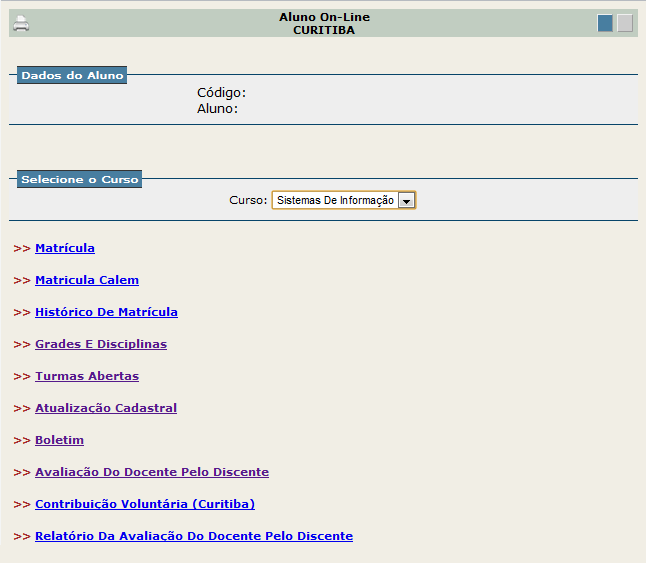
\includegraphics[scale=0.5]{Menu_Principal_1.png}
		\caption{Menu Principal}
		\label{menuPrincipal}
	\end{figure}

Para saber as disciplinas da grade do seu curso e seus respectivos códigos, você deve entrar no menu ``Grades e Disciplinas'' e selecionar Engenharia / Bacharelado  (Figura  \ref{gradeMenu}). Se a grade não for especificada, uma tela como a da Figura  \ref{gradeTabela} irá aparecer, e você poderá selecionar a grade que deseja consultar. O código da Grade de Sistemas de Informação é 597 e de Engenharia de Computação é 544.

	\begin{figure}[ht!]  \centering
		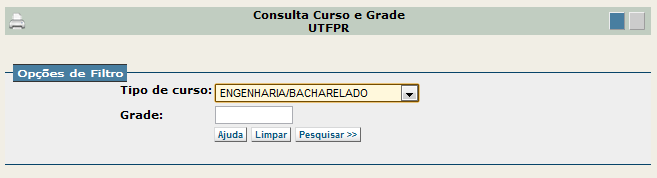
\includegraphics[scale=0.5]{Grade_Menu.png}
		\caption{Menu Grades e Disciplinas}
		\label{gradeMenu}
	\end{figure}

	\begin{figure}[ht!]  \centering
		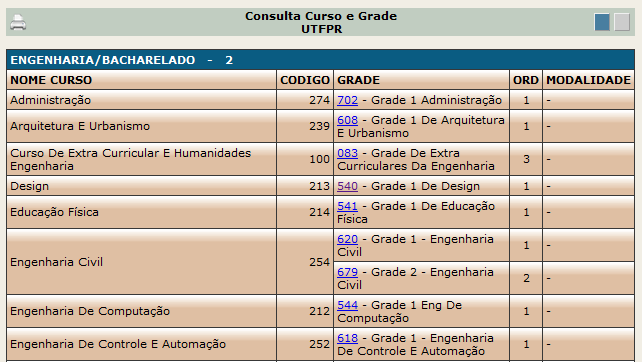
\includegraphics[scale=0.5]{Grade_Tabela.png}
		\caption{Tabela de Grades de Engenharia/Bacharelado}
		\label{gradeTabela}
	\end{figure}

Isso feito, você terá acesso a informações valiosas, como as disciplinas a serem cursadas em cada período. Além disso, para cada disciplina, estão listados o código; número de créditos; carga horária prática,teórica, semanal e total; disciplina que é pré-requisito ; disciplina equivalente e se a disciplina em questão é obrigatoria ou optativa. Na Figura \ref{gradeCurso} está representada a grade de Sistemas de Informação.

	\begin{figure}[ht!]  \centering
		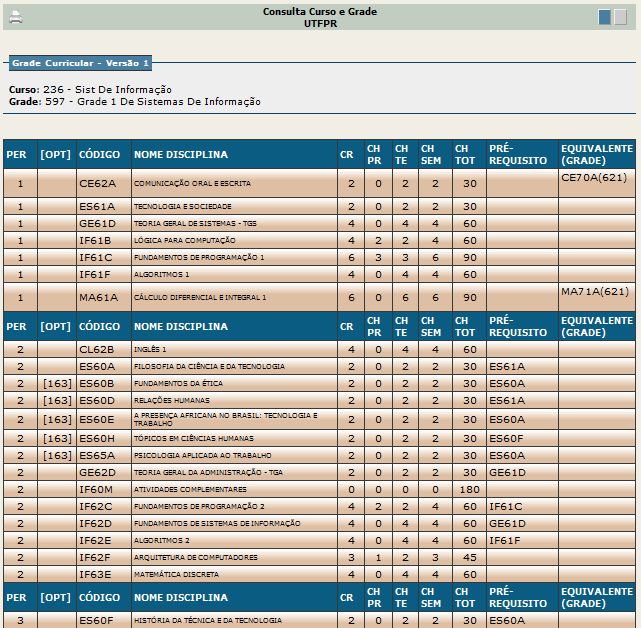
\includegraphics[scale=0.5]{Grade_Curso.png}
		\caption{Grade 597 - Sistemas de Informação}
		\label{gradeCurso}
	\end{figure}

Isto feito, você pode consultar as turmas abertas de cada disciplina. Para isso, abra uma nova janela no navegador, e no Menu Principal clique em ``Turmas Abertas'' e escolha seu curso. No exemplo utilizamos o 236 - Sistemas de Informação (Engenharia da computação é o curso 212) - Figura \ref{turmasAbertasMenu}.

	\begin{figure}[ht!]  \centering
		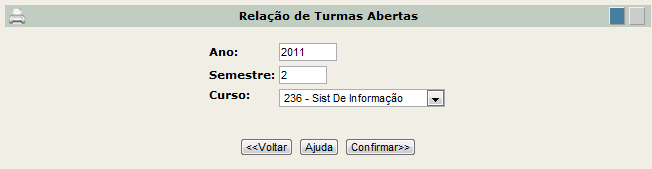
\includegraphics[scale=0.3]{Turmas_Abertas_Menu.png}
		\caption{Menu de Turmas Abertas}
		\label{turmasAbertasMenu}
	\end{figure}

Ao confirmar a escolha do curso, uma relação das turmas de cada disciplina irá aparecer (Figura \ref{turmasAbertasTabela}). A seguir explicamos o que significa cada coluna:

\begin{itemize}
\item Turma: Identifica o Curso e o tipo de turma. S01 e S02 são para Turmas Especiais. S71 e S72 são Turmas do curso de Eng. de Computação e S73 Turmas de Sistemas de Informação.

\item Vagas Totais: depende da capacidade dos laboratórios/ salas de aula.

\item Vagas Calouros: S indica uma turma de calouros; N indica uma turma de veteranos.

\item Reserva: S para Sem Reserva (pessoas de todos os cursos podem entrar, sem restrições), A para Aberta (para alunos de todos os cursos, porém com prioridade para alguns) e F para Fechada (somente para alunos do curso em questão).

\item Curso: indica os cursos aos quais a disciplina é dirigida, em ordem de prioridade.

\item Horário: o horário é representado da seguinte forma: dia/turno/aula. Assim, 3T1 significa terça-feira à tarde primeiro horário (no caso 13h).

\item Professor: nome do professor previsto para a turma

\item Optativa: indica se a disciplina é optativa.

\end{itemize}

	\begin{figure}[ht!]  \centering
		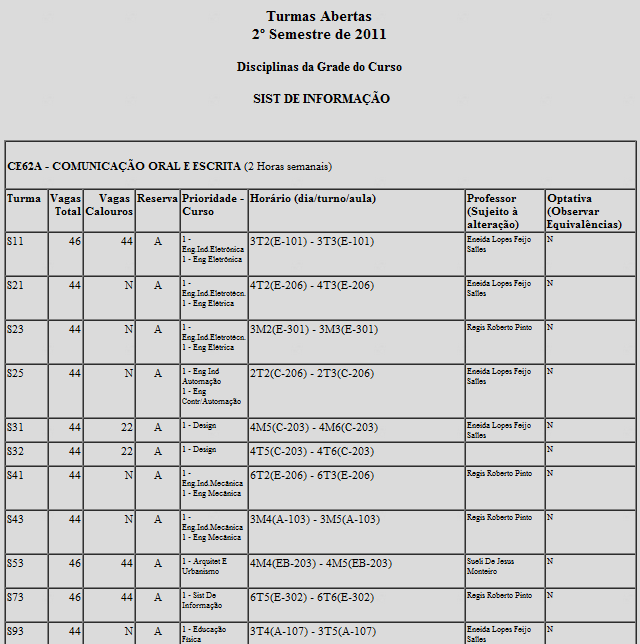
\includegraphics[scale=0.5]{Turmas_Abertas_Tabela.png}
		\caption{Relação de Turmas Abertas de Sistemas de Informação}
		\label{turmasAbertasTabela}
	\end{figure}

Depois de todas essas consultas, está na hora de montar o seu horário, não acha?! Se você está com preguiça de abrir o Excel, ou até mesmo de pegar uma folha e caneta para isso, indicamos a ferramenta \href{http://www.caiux.net/utfpr/}{Grade Fácil}, desenvolvida pelo aluno  da UTFPR.

Com os códigos das disciplinas e das turmas que você pretende cursar em mãos, FINALMENTE chegou a hora de realizar o requerimento. No menu principal, clique em ``Matrícula''. Uma página como a da Figura \ref{matriculaRequerimentoPreenchido} irá aparecer. Basta preencher com o código da disciplina e respectiva turma.

	\begin{figure}[ht!]  \centering
		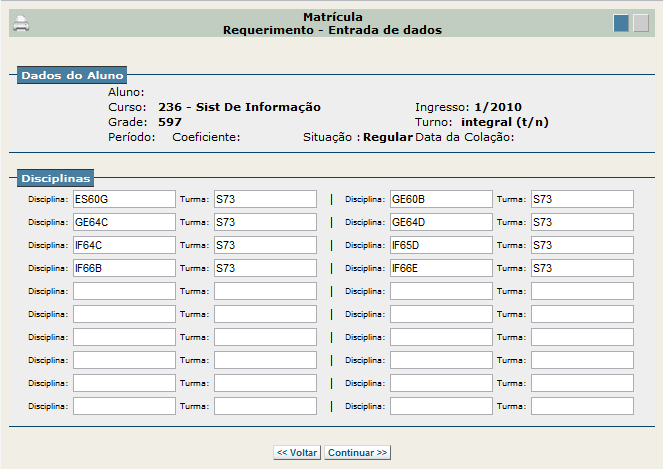
\includegraphics[scale=0.5]{Matricula_Requerimento_Preenchido.png}
		\caption{Requerimento de Matrícula Preenchido}
		\label{matriculaRequerimentoPreenchido}
	\end{figure}

Ao clicar em continuar, aparecerá uma tela que mostra se o requerimento pode ser enviado (não tem problemas de validação) - Figura \ref{matriculaRequerimentoResultadoParcial}. Se estiver tudo como você tinha planejado, é só clicar em ``Finalizar Matrícula'' e imprimir o ``comprovante'' (Figura \ref{matriculaRequerimentoAceito}).

	\begin{figure}[ht!]  \centering
		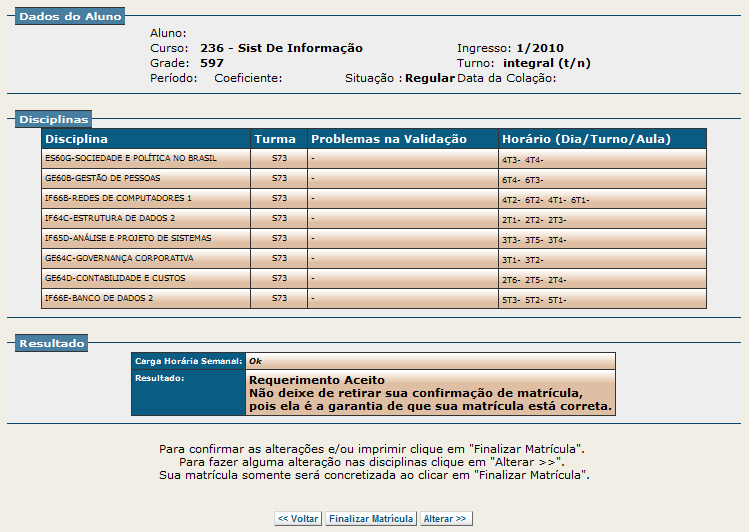
\includegraphics[scale=0.5]{Matricula_Requerimento_Resultado_Parcial.png}
		\caption{Requerimento de Matrícula - Resultado Parcial}
		\label{matriculaRequerimentoResultadoParcial}
	\end{figure}

	\begin{figure}[ht!]  \centering
		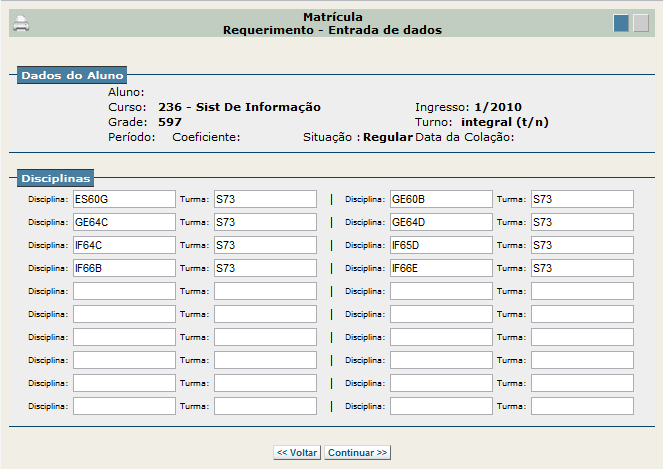
\includegraphics[scale=0.5]{Matricula_Requerimento_Preenchido.png}
		\caption{Requerimento de Matrícula Aceito}
		\label{matriculaRequerimentoAceito}
	\end{figure}


\subsection{Confirmação e Ajuste}


\subsection{Inclusão}



\end{document}
